\chapter{Implementácia}\label{chap:implementation}
Kapitolu sme zamerali na opis implementácie webovej aplikácie, časti interpretera - verifikátoru UNITY a dostupných knižníc S2N, 
NuSMV.

\section{Aplikácia}
Prostredie pre vytvorenie samotnej aplikácie sme si zvolili webovú stránku. Táto stránka okrem aplikácie je 
uvádzaná aj ako prezentačná stránka našej diplomovej práce. Obsahuje všetky základné informácie o práci, 
postupe a zdrojov. Hlavná časť stránky je zameraná samotnej aplikácií teda verifikátoru pre UNITY. Aplikácia 
sa skladá z interpretera a knižníc S2N, NuSMV. Na zápis programu UNITY sme použili jednoduchý code editor,
ktorý sa nachádza na podstránke Aplikácia, ktorú môžete vidieť na obrzázku \ref{img:web}.

\subsection{Back-end}
Pre server-side sme si zvolili jazyk GO, známy aj ako Golang. Je to typovo orientovaný, kompilovateľný 
programovací jazyk, ktorý navrhol Google. Golang je syntakticky veľmi podobný jazyku C. Samotný jazyk je 
pôvodne navrhnutý na vývoj webových aplikácií, avšak dá sa použiť rôzne. Nás osobne veľmi zaujal a tak sme si ho
vybrali na vývoj aplikácie.

\subsubsection{Web framework}
Golang sám o sebe sa dá použiť bez akýchkoľvek framework-ov na vývoj webových aplikácií. Avšak takáto 
implementácia je obzvlášť zložitá z dôvodu rôznych modulárnych knižníc. Preto sme sa rozhodli použiť už 
existujúci web framework Buffalo. Tento framework je jednoduchý a pri tom výkonný na tvorbu web-u. 

\subsection{Front-end}
Použili sme HTML5/CSS3 s pomocou React komponentov. Jednotlivé podstránky sú tvorené z HTML súborov, ktoré
obsahujú React komponenty, tie nám zaručujú real-time rendering. 

\subsubsection{React}
Je JavaScript-ová knižnica, ktorá dokáže v reálnom čase vykresľovať dané komponenty bez akéhokoľvek refreshu
stránky. Časti stránky obsahujú dva zložitejšie komponenty: časovú os postupu práce a code editor.

\subsection{Server - Heroku}
Web framework Buffalo je už od začiatku vytvorenia nového projektu pripravený na nahratie na server. K tomu
používa systém Heroku. Heroku je cloud-ová služba na správu webových aplikácií. Preto sme túto možnosť využili
a celú aplikáciu sme nahrali na Heroku server. Aplikácia je neustále dostupná na tomto 
\href{https://spaldon-diplomovka.herokuapp.com}{LINKU}.

\subsubsection{Zdrojové súbory aplikácie}
Pre prípad potreby sme celú aplikáciu uložili na stránke \href{https://github.com/FiFOOO/unity_verificator}{GITHUB}. 
Je potrebné mať nainštalovaný Golang a preň framework Buffalo. Samotný server sa spustí príkazom 
\texttt{buffalo dev}.


\begin{figure}[H]
    \centerline{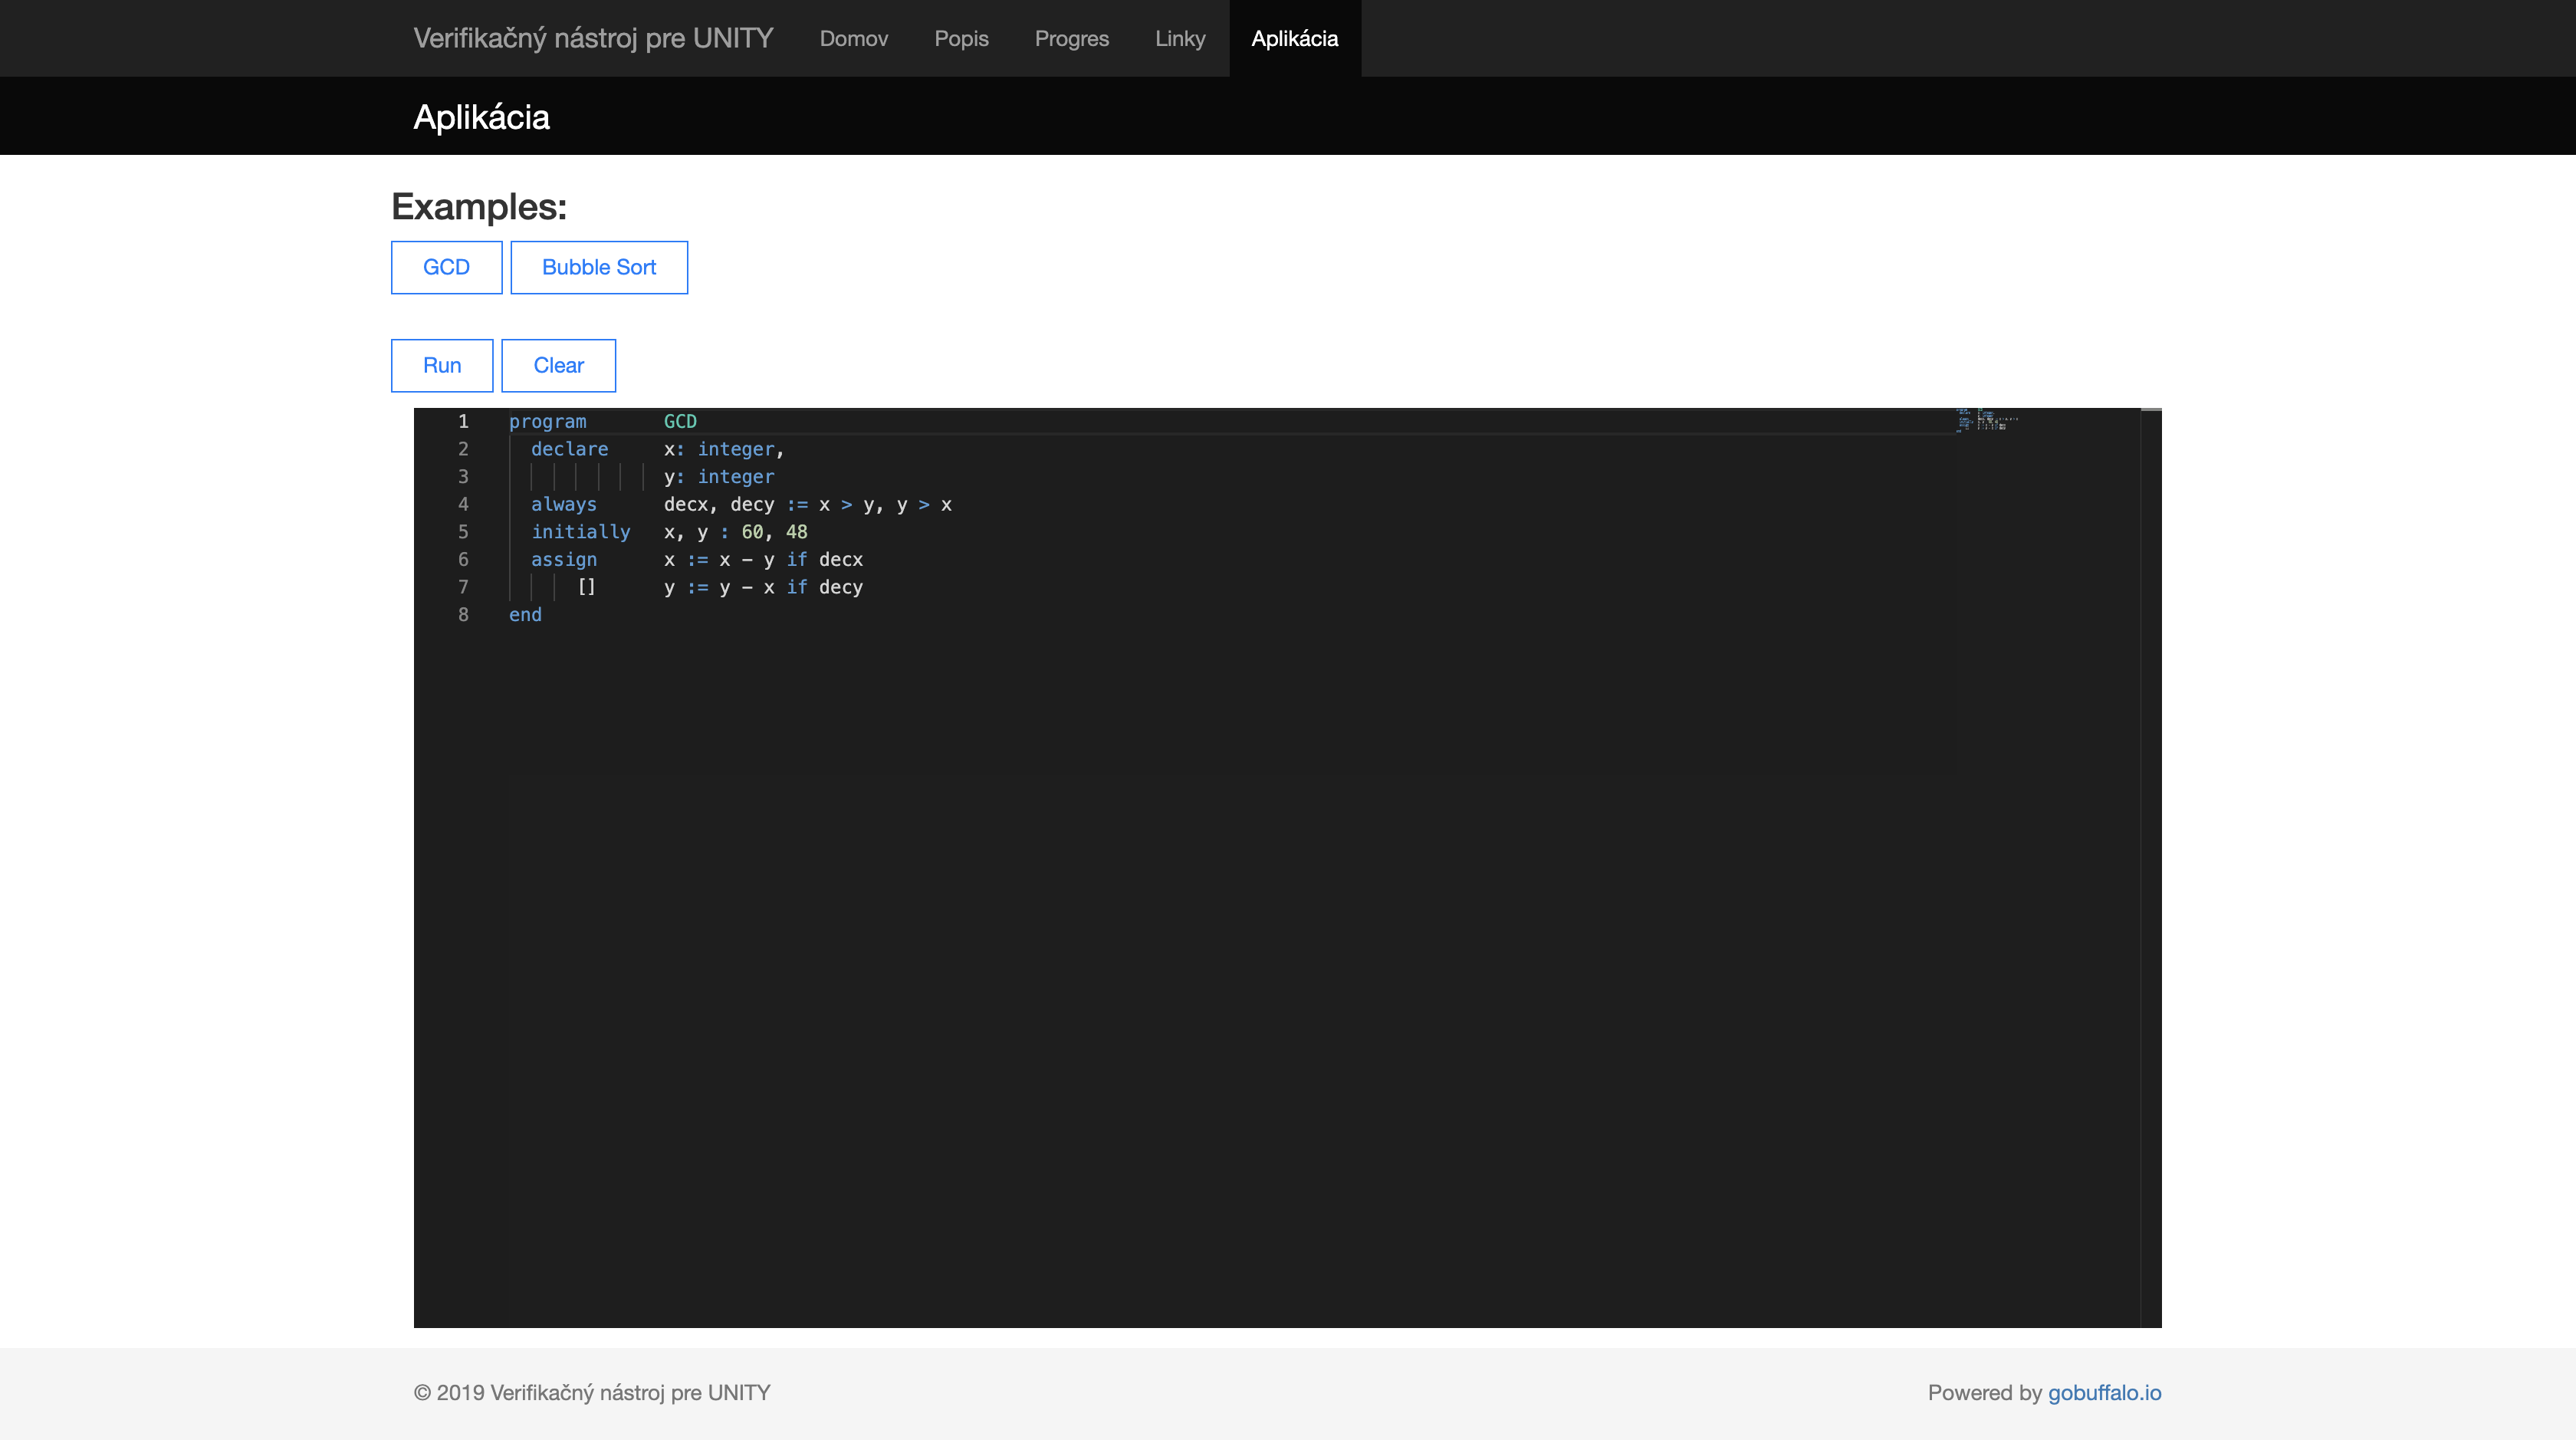
\includegraphics[width=1\textwidth]{images/web}}
    \caption[Podstránka Aplikácia]{Podstránka Aplikácia}
    \label{img:web}
\end{figure}

\section{Implementácia interpretera}
Náš interpreter obsahuje lexikálnu analýzu, syntaktickú analýzu a generátor cieľového kódu. 


\subsection{Lexikálna analýza}
Táto časť interpretera je najdôležitejšia, pretože načítava vstupný text programu UNITY. Text sa zadáva
do code editor-u. Editor obsahuje dve hlavné tlačidlá RUN a CLEAR. RUN spustí samotný interpreter a CLEAR
vyčistí obsah code editor-a. 

Keď sa celý proces spracovania textu začne vytvorí sa trieda \texttt{Unity} (obr. \ref{img:unity}), ktorá je 
jadrom interpretera. Táto trieda má niekoľko funkcií ale najdôležitejšou je funkcia \texttt{Parse}, 
ktorá využíva funkcie \texttt{Next} a \texttt{Scan}. Spolupráca \texttt{Next} a \texttt{Scan} nám vracia 
token-y, ktoré predstavujú buď čísla, slová (premenné, časti programu) alebo symboly (operátory). 

\texttt{Parse} prechádza text postupne po sekciách programu a zapisuje jednotlivé premenné do lokálnej 
premennej \texttt{Variables}. Tieto premenné sú deklarované v sekcii \textbf{declare} programu UNITY. 
Ak program obsahuje aj sekciu \textbf{always}, tak jej transparetné premenné sa tiež pridajú k \texttt{Variables}.
Následne prechádzame do sekcie \textbf{initially}. Okrem toho, že \texttt{Parse} kontroluje správnu syntax
textu, zároveň kontroluje či dané premenné sú správne deklarované a počas vykonávania sekcie \textbf{initially}
overuje, že tieto premenné boli aj správne inicializované. \textbf{Assign} sekcia je špeciálna tým, že 
obsahuje príkazy, ktoré predstavujú chod celého programu. Je to časť, kde sa využívajú všetky deklarované a
inicializované premenné aby dosiahli nejakého výsledku. Preto sa jednotlivé príkazy pridávajú do lokálnej
premennej \texttt{Body}. \texttt{Body} je tzv. array of dictionaries (pole slovníkov), 
ktoré okrem sekcii \textbf{assign} obsahuje aj ostatné sekcie. Kľúčom pre tieto slovníky sú názvy sekcií, 
hodnotou sú priradenia danej sekcie. Táto premenná sa ďalej používa v syntaktickej analýze

\begin{figure}[H]
    \centerline{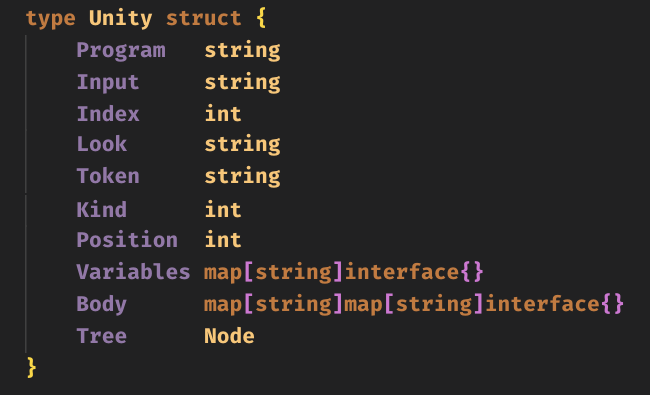
\includegraphics[width=0.5\textwidth]{images/unity}}
    \caption[Trieda Unity]{Trieda Unity}
    \label{img:unity}
\end{figure}

\subsection{Syntaktická analýza}
Syntaktická analýza má jednu dôležitú úlohu a to z celého programu UNITY vytvoriť abstraktný syntaktický strom.
AST musel obsahovať všetky sekcie aby sme dokázali vygenerovať cieľový kód. Analyzátor využíva lokálnu 
premennú \texttt{Body}. Postupne prechádza každú sekciu a vytvára z nej AST. Avšak pri niektorých sekciách to
bolo obzvlášť náročné. 

K vytvoreniu AST nám pomáhala trieda \texttt{Node} (obr. \ref{img:node}). Obsahujúca niekoľko premenných, ktoré
nám hovorili čo daný \texttt{Node} predstavuje. Napr. ak premenná \texttt{Statement} obsahovala nejakú hodnotu,
tak to vždy bol \texttt{string}, hovoriaci čo sa bude diať s jeho podstromami. Mohla obsahovať 
\texttt{=, -, +, *, /, <, >, <=, >=, ==, !=}.

\begin{figure}[H]
    \centerline{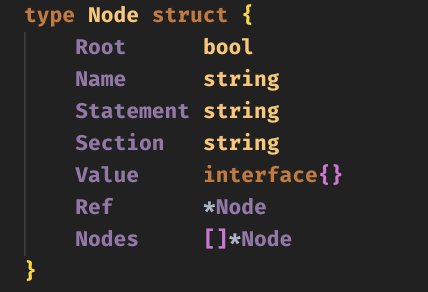
\includegraphics[width=0.5\textwidth]{images/node}}
    \caption[Trieda Node]{Trieda Node}
    \label{img:node}
\end{figure}

Sekcia \textbf{always} môže obsahovať už zložitejšie výrazy napr.
\texttt{decx, decy := x > y, y > x}. Premenná \texttt{decx} predstavuje výraz \texttt{x > y}. 
Takýto výraz sme museli rozdeliť na tri časti: podstrom kde \texttt{Statement} sa rovnal operandu 
\texttt{>} a jeho listy. Ľavým listom bola hodnota \texttt{x} a pravým listom hodnota \texttt{y}. 
Na vytvorenie podstromu v sekcii \textbf{always} sme používali pomocnú funkciu \texttt{makeAlwaysNode}.

\textbf{Initially} obsahuje aj kvantifikované priradenia a výrazy. Príkladom je 
\texttt{<|| k: 0 <= k < N :: A[k] = rand() >}. Toto priradenie hovorí, že sa má pole \texttt{A} naplniť
náhodnými hodnotami. Ľavá strana od znaku \texttt{::} predstavuje for-cyklus od \texttt{0} po \texttt{N} 
a pravá strana samotné priradenie náhodnej hodnoty pre daný index poľa. Keď sme chceli priradenie zapísať 
do stromu museli sme pole A vytvoriť a inicializovať (obr. \ref{img:for}). Ľavú stranu sme 
inicializovali funkciou \texttt{forParserLeft}, ktorá nám vrátila iteráciu od \texttt{0} po \texttt{N}.
Pole \texttt{A} sme potom vytvorili za pomoci \texttt{forParserRightInitially}.

\begin{figure}[H]
    \centerline{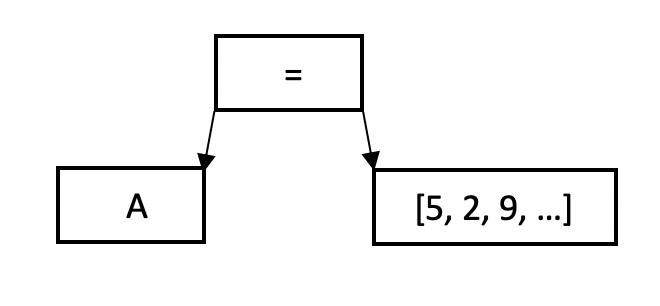
\includegraphics[width=0.5\textwidth]{images/for}}
    \caption[Initially - Pole A]{Initially - Pole A}
    \label{img:for}
\end{figure}

Ak išlo o sekciu \textbf{assign} tá obsahovala príkazy - množinu priradení. Priradenia sme museli rozdeľovať
na bežné a kvantifikované. Bežné sme zapisovali ako rovnosť ľavej a pravej strany, avšak pravá strana mohla 
obsahovať podmienku \texttt{if}. Podmienka bola priradená do \texttt{Node} ako referencia (\texttt{Ref}).
Kvantifikované priradenia sme vytvorili ako for-cyklus so svojimi jednotlivými priradeniami (obr. \ref{img:for2}). 

\begin{figure}[H]
    \centerline{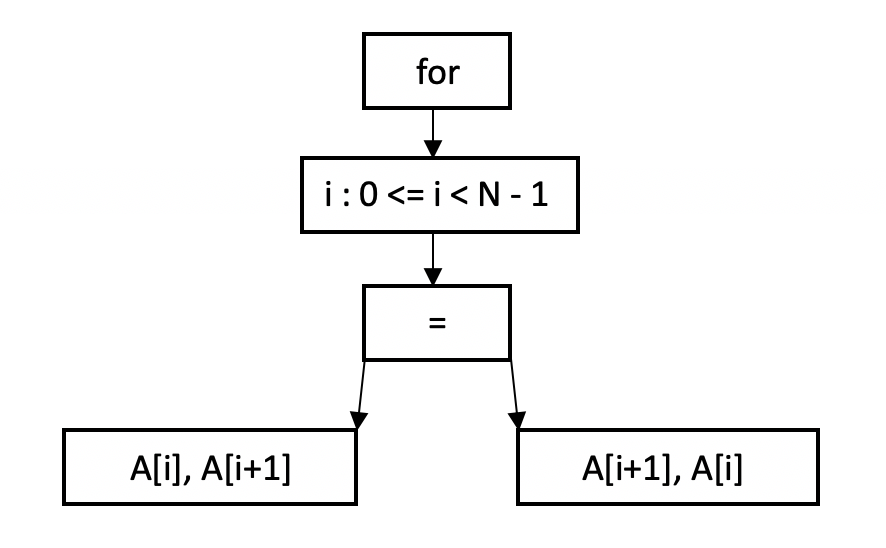
\includegraphics[width=0.6\textwidth]{images/for2}}
    \caption[Kvantifikované priradenie v AST]{Kvantifikované priradenie v AST}
    \label{img:for2}
\end{figure}

\subsection{Generátor cieľového kódu}
V tomto okamihu sme už mali vytvorený AST, ktorý sme museli následne transformovať do cieľového kódu. 
Pre vytvorenie kódu sme využili funkciu \texttt{MakePromela}. 

Na prechádzanie stromu sme použili algoritmus DFS (Depth-first search). Postupne sme zapisovali do lokálnej
premennej \texttt{pom} všetky sekcie programu. Deklarované premenné sme definovali ako globálne premenné, 
pričom sme ich museli inicializovať v časti \texttt{init}. Nástroj S2N nepodporuje inicializácie 
globálnych premenných. Ako sme už spomínali bolo potrebné aby sa všetky priradenia vykonávali 
paralelne a preto sme každé priradenie z množiny priradení sekcie \textbf{assign} definovali 
ako \texttt{active proctype} s názvom \texttt{process\_index\_procesu}. Pre zabezpečenie nekonečného 
vykonávania sme priradenia vložili do cyklu za pomoci \texttt{do}. Musel ale obsahovať podmienku 
\texttt{:: else -> skip}, ktorá finálne zabezpečila nekonečné vykonávanie každého priradenia. 
Keďže sa priradenia vykonávali paralelne a používali rovnaké premenné nastávala situácia, že sa niektoré
priradenia premenných vykonávali zle a nadobúdali zlé hodnoty. Museli sme preto použiť atomické operácie.

Výsledný kód bol zapísaný v jazyku Promela do súboru \texttt{program.pml}. Ukážku môžete vidieť na obr. 
\ref{img:gcd}.

\begin{figure}[H]
    \centerline{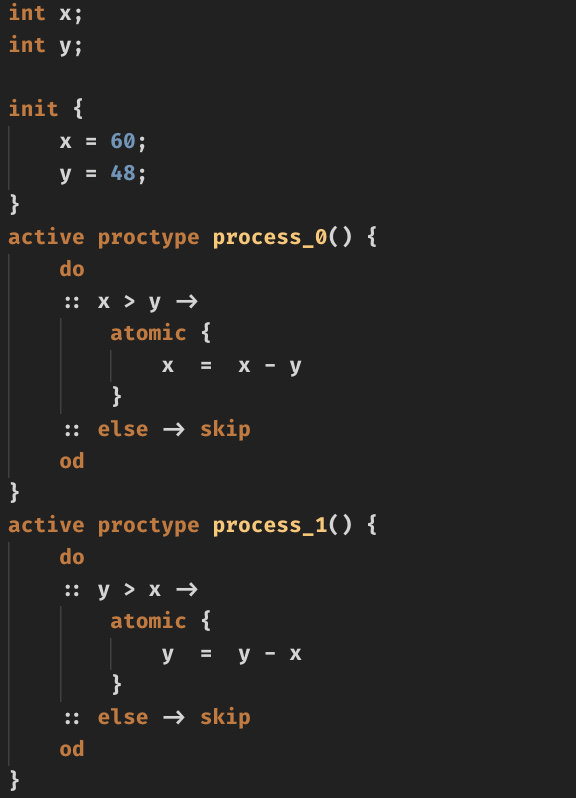
\includegraphics[width=0.5\textwidth]{images/gcd}}
    \caption[GCD v jazyku Promela]{GCD v jazyku Promela}
    \label{img:gcd}
\end{figure}


\section{Verifikácia programu}
Po vložení programu UNITY do code editor-u a stlačení tlačidla RUN sa program spracuje. Výsledkom 
procesu je súbor \texttt{program.smv}. Tento súbor sa vygeneruje za použitia nástroja S2N, ktorý
upraví súbor \texttt{program.pml}. 

Pre verifikáciu programu sme použili model checker NuSMV. Pretože 
NuSMV používa svoj vlastný interaktívny shell nebolo možné proces verifikácie zahrnúť do vytvorenej aplikácie.

NuSMV je dostupný v zložke projektu \texttt{bin}, kde sa nachádza aj nástroj S2N. Výstupný súbor 
\texttt{program.smv} si buď stiahnete po vykonaní aplikácie alebo ho môžete nájsť v zložke \texttt{public/out/}.

Pre spustenie verifikátoru NuSMV je potrebné vykonať príkaz \texttt{bin/NuSMV -int public/out/program.smv} z
koreňu projektu. Následne sa spustí interaktívny shell, kde už začína verfikácia vlastností programu UNITY.

Ukážku shell-u po simulovaní troch krokoch môžete vidieť na obr. \ref{img:nusmv1} a \ref{img:nusmv2}.


\begin{figure}[H]
    \centerline{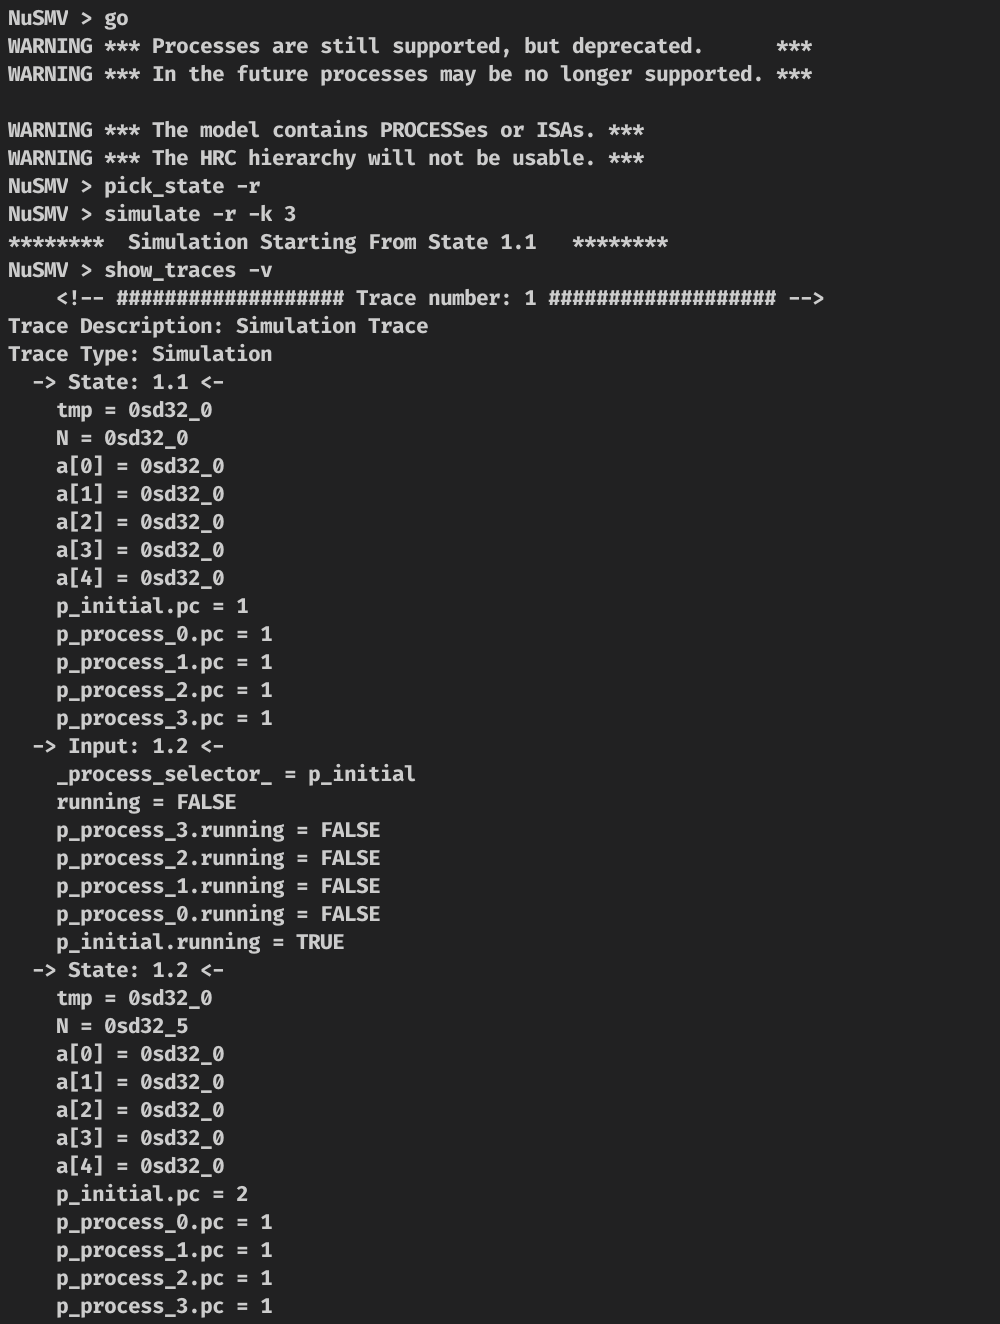
\includegraphics[width=0.4\textwidth]{images/nusmv1}}
    \caption[Prvá časť simulácie NuSMV]{Prvá časť simulácie NuSMV}
    \label{img:nusmv1}
\end{figure}

\begin{figure}[H]
    \centerline{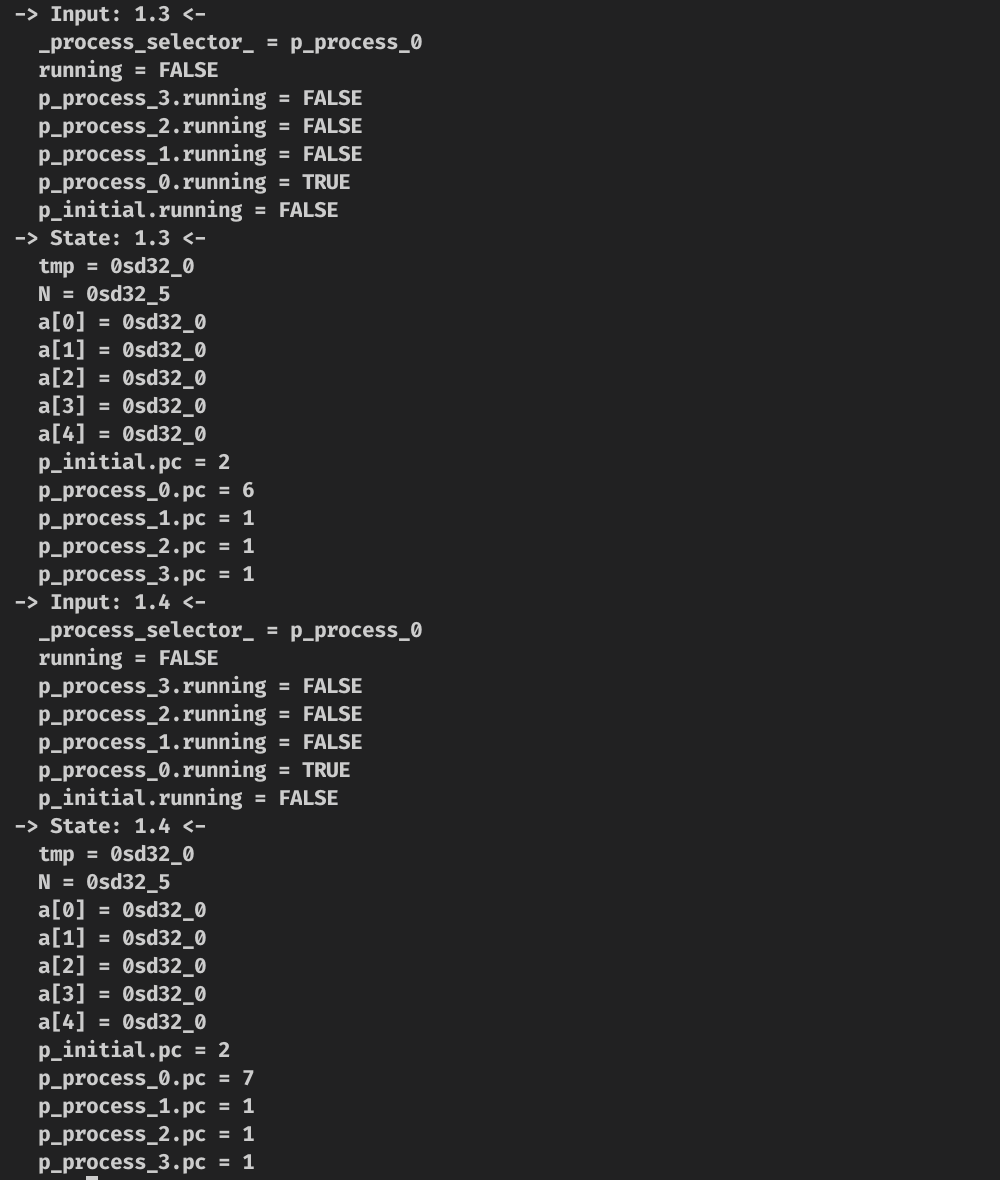
\includegraphics[width=0.4\textwidth]{images/nusmv2}}
    \caption[Druhá časť simulácie NuSMV]{Druhá časť simulácie NuSMV}
    \label{img:nusmv2}
\end{figure}